

The EUTelescope package \cite{ref:eutelwebsite} provides software tools for offline analysis and reconstruction of telescope test beam data. 
EUTelescope is embedded into the ILCSoft framework~\cite{ref:eudetmemo_2009_12} which provides the basic building blocks for offline analysis such as a data model (Linear Collider I/O, \emph{LCIO}),
a geometry description language (\emph{GEAR}) and the central event processor (\emph{Marlin}).

% thomas: this should be a reference to ilcsoft, not: \cite{EUDET-2008-48}.

EUTelescope comes with its own job submission framework \emph{jobsub} that allows to run analysis jobs locally or to submit them to larger computing clusters such as NAF.

Marlin allows the modular composition of analysis chains for various applications since every task is implemented as an independent \emph{processor} that is called by Marlin. 
The processors expose a set of parameters to the user which can be configured and loaded at runtime via so-called \emph{steering files} in XML format.
This way the Marlin/Processor architecture gives a lot of flexibility to the end user. 

EUTelescope provides several processors for Marlin implementing algorithms necessary for a full track reconstruction and data analysis of beam test experiments. 
%Figure~\ref{fig:offline:strategy} shows the analysis strategy of the framework starting from the recorded detector response to the final aligned particle tracks. 
%An overview of the processor range provided by EUTelescope is given in \cite{EUDET-2007-20}.
For low-energy beams such as the DESY-II test beam facility multiple scattering is the dominating source of track resolution uncertainties. 
Therefore EUTelescope provides advanced algorithms such as General Broken Lines (GBL) \cite{Kleinwort-2012} for tracking which accounts for scattering in all material present in the beam. 
In addition, precise software alignment can be performed using the Millipede-II algorithm \cite{Blobel-2006}.

\label{sec:datura-nodut}
Within EUTelescope, an example set of processors and configurations were created as an introduction for new users to EUTelescope.
This example is called \texttt{datura-noDUT}, since no user DUT is included.
Two GEAR files are provided, for different telescope geometries.
No external device under test is used, only the six MIMOSA 26 telescope planes are included.
The goal of the \texttt{datura-noDUT} example is to get from raw detector data to unbiased track residuals of each telescope plane.

The \texttt{datura-noDUT} example is constructed such, that a certain sequence of steering files is called.
After all steps have been applied on a run, the unbiased residuals for this run should have been successfully calculated.
An overview of the steps is shown in figure~\ref{fig:datura-nodutsequence}.

\begin{figure}[tbp]
  \centering
  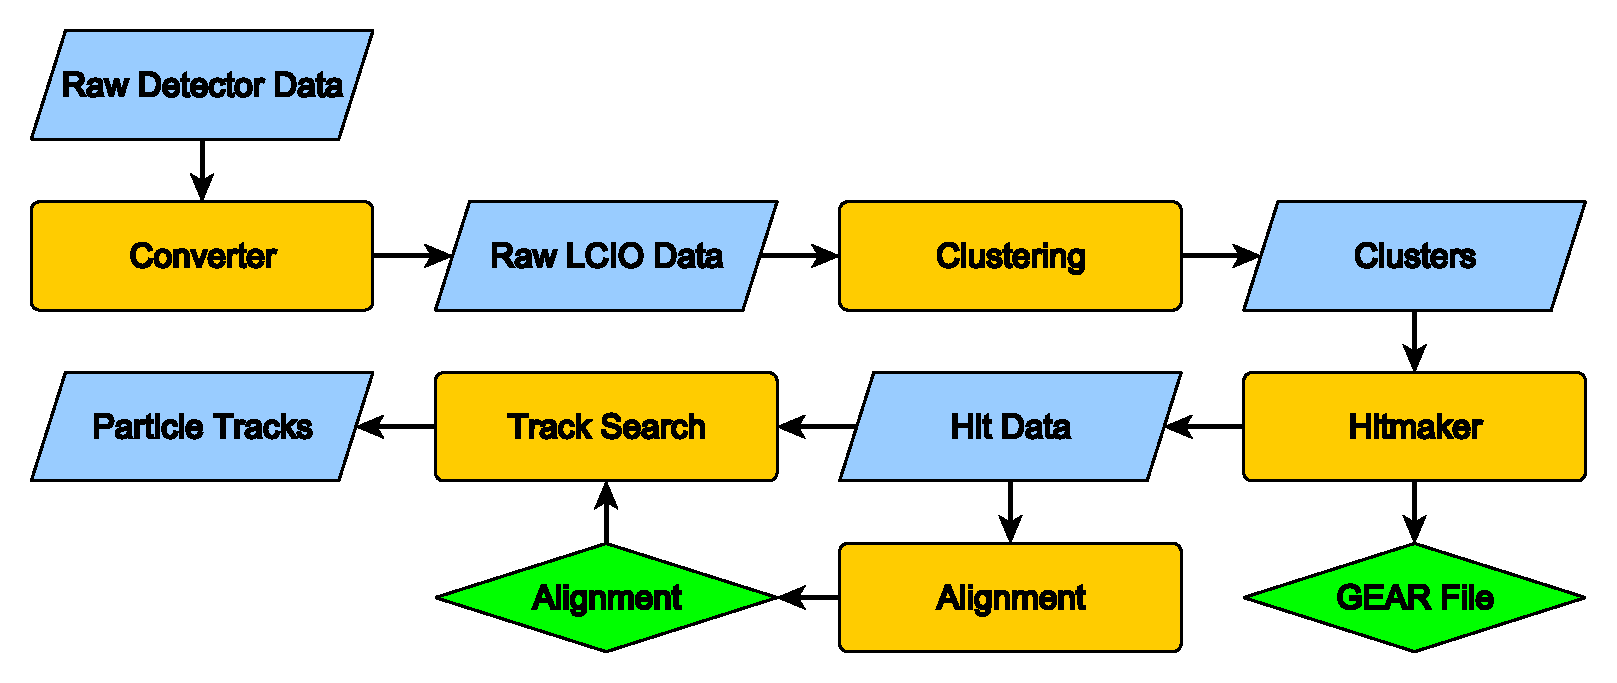
\includegraphics[width=0.9\textwidth]{figures/datura-noDUT_paper}
  \caption[Steps performed in the \texttt{datura-noDUT} example]{Sequence of the steps performed in the \texttt{datura-noDUT} example. 
  Data states are indicated blue, external files green. \\comment hjansen: What is yellow? Converter? Why ``alignment'' as external file and yellow?}
  \label{fig:datura-nodutsequence}
\end{figure}

The first steering file called is the converter.
Its goal is to convert the raw MIMOSA 26 detector data into the LCIO format and remove any noisy pixels.
Following the converter, the clustering is performed.
Clusters are searched on each telescope plane and written to an LCIO collection.
A preliminary correlation is calculated and can be used for debugging purposes.
The hitmaker step transforms the clusters from two-dimensional entities on a telescope plane into hits in a global three-dimensional frame.
A rough pre-alignment is calculated and stored in a database file.

For the alignment two separate methods are available - either a simple straight line tracking or an implementation of the deterministic annealing filter (DAF) fitter~\cite{ref:daffitter}.
In both cases, the pre-alignment is loaded and applied to the hit data.
Tracks are searched and passed to \texttt{MillepedeII}~\cite{Blobel-2006} to determine the alignment constants.
These constants are then stored in another database file.

The final fitter step calculates the unbiased residual distribution for each telescope plane.
The prealignment and alignment are loaded and applied to the hit collections.
Once again, tracks are searched, but with one telescope plane considered passive, thus not contributing to the track fit.
Instead, the track is extrapolated to this plane, and the residual distance to this plane's hits is calculated.
This is repeated for each telescope plane, with histograms written to \texttt{ROOT} files.


